\section{End Flag Generator}

To generate a valid \(end\_flag\) signal for the ALU, a Timed Mealy State Machine is introduced into the circuit.
For instance, a pipelining circuit will result in the output after counting 4 synchronized clock cycles
when the \textquote{load} signal goes from high to low. The counting of the clock cycle is implemented by rotating a
vector signal to avoid inrtoducing extra addition circuit.

The ASMD chart is presented in \figref{fig:asmd}.
And the RTL description of the generator is presented in \figref{fig:end_flag_gen_rtl}.

\begin{figure}[!ht]
	\centering
	\caption{ASMD Chart of the FSM of the 4 Stage End Flag Generator}
	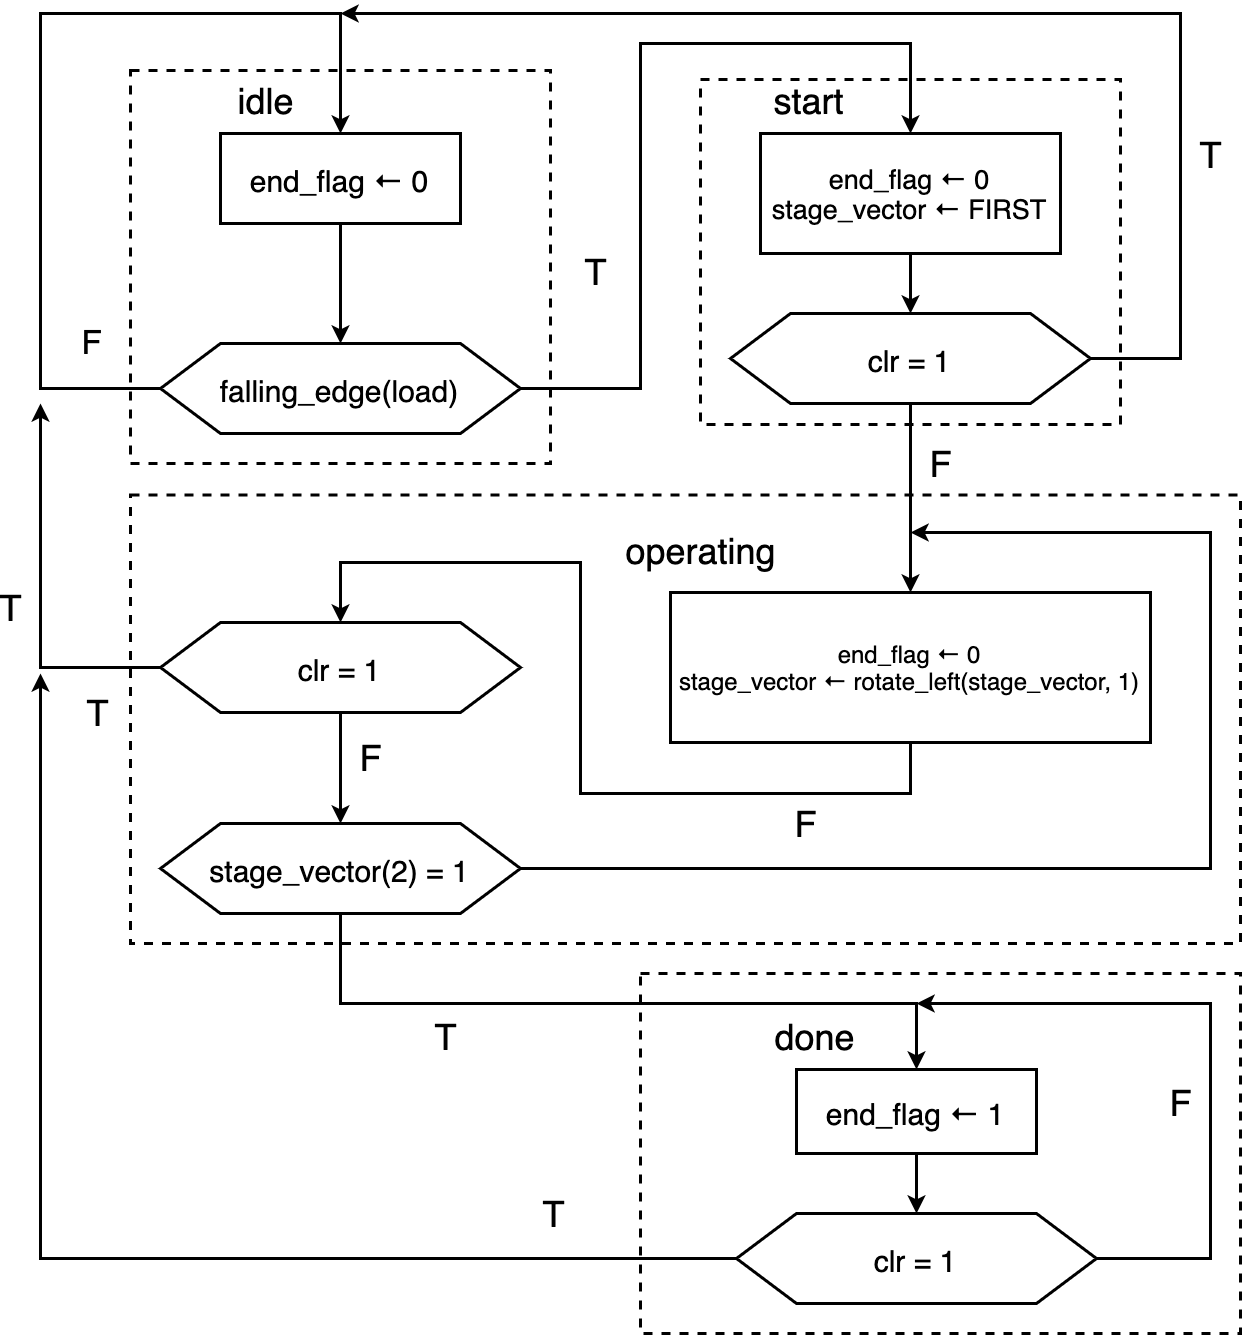
\includegraphics[width=0.7\textwidth]{../img/asmd.png}
	\figurenote{\textquote{stege\_vector} is a 4 bit vector signal; \textquote{FIRST} is \textquote{0001}.}
	\label{fig:asmd}
\end{figure}

\begin{figure*}[!ht]
	\centering
	\caption{Synthesized RTL Diagram of End Flag Generator for 4 Operation Stages}
	\includegraphics[height=0.9\textheight]{../img/end_flag_gen_rtl.png}
	\label{fig:end_flag_gen_rtl}
\end{figure*}
